\section{Linear Feedback Shift Register (LFSR)}
El \textit{Linear Feedback Shift Register} es un registro de desplazamiento en el que la entrada se calcula a través de una función lineal. Uno de sus usos es cifrar una secuencia binaria (a traves de la suma de un \textit{keystream} a los datos en claro), o para generar una secuencia aleatoria de dígitos a partir de una semilla o estado inicial. A la función que describe el calculo de la siguiente entrada del registro también se la conoce como polinomio de \textit{feedback}.  %no estoy seguro de si necesitabas la secuencia inicial para el crack% \\\\
Para ser más precisos teniendo una cadena binaria $b$.
\[ b = b_0, b_1, ... , b_n\]
Siendo \(n\) el numero de bits del estado inicial del LFSR, se aplicará sobre esta cadena un xor sobre ciertas posiciones de tal manera que nos de como output el bit en la posicion 0, del nuevo estado de la cadena/secuencia. A las posiciones sobre las que se aplica el xor se les llama según la literatura científica \textit{taps}.

Así que teniendo la secuencia $b$. Y por ejemplo, \textit{taps} en las posiciones 0, 1 y 4. Siendo \(b>=4\). El siguiente estado de la secuencia se computará de esta manera
\[ output = b_0 \oplus b_1 \oplus b_4 \]
\[ b = output, b_0, b_1, b_2, b_3, b_4, ..., b_{n-1}\]

Con imágenes se ve mucho más claro la naturaleza del LFSR como proceso recursivo. Pongamos como ejemplo la secuencia ``0100``, y pongamos como \textit{taps} la posición 0 y la posición 1. \\ 
\begin{figure}[h] 
    \centering
    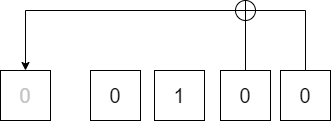
\includegraphics[width=0.5\textwidth,keepaspectratio]{img/lfsr_01.png} .
    \label{fig:mi_imagen}
\end{figure}
\\
En la figura, se aprecia como el XOR entre la posición 0 de la cadena binaria, y la posición 1, resulta en el bit que ocupará la posición 3 de la cadena. Todos los bits del estado anterior se desplazan una posición hacia la derecha eliminando el bit en posicion 0 del estado anterior. Y por último se repite, la operación XOR.
\newpage
\begin{figure}[h] 
    \centering
    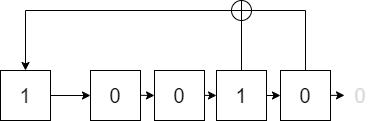
\includegraphics[width=0.5\textwidth,keepaspectratio]{img/lfsr02.png} .
    \label{fig:mi_imagen}
\end{figure}
\noindent El polinomio del LFSR del ejemplo, es un polinomio primmitivo ya que para que el registro vuelva a tener el valor de la semilla es necesario hacer $2^n-1$ iteraciones, ese menos uno se debe a que evidentemente el registro no puede valer 0 ya que en ese caso sin importar el número de iteraciones siempre permanecería en 0.\\\\
Para concluir esta sección y esclarecer del todo este tema de los registro de desplazamiento, en la siguiente figura tenéis un pseudocódigo naive para implementar cualquier LFSR.\\ 
\begin{algorithm}
\caption{Algoritmo lfsr(s, t, k)}\label{alg:zero}
\KwData{$s$ = secuencia binaria, $t$ = lista con las taps positions, k = numero de steps/iteraciones}
\KwResult{s después de k iteraciones}
\For{$i = 0; i < k; i++$}{
    $output \gets s[taps[0]]$\;
    \For{$j = 0; j < len(t); j++$} {
        $output \gets output \oplus s[taps[j]]$\;
    }
    $s = output, s[len(s)-1]$\;
}
\end{algorithm}
\\
Cabe destacar, lo increíblemente simple que es, para lo complejos que pueden llegar a ser los output a los que da salida este algoritmo. Aunque existen técnicas para decodificar estas secuencias y obtener tanto el polinomio como el estado inicial. %La implementación es extremadamente rápida en hardware ya que las operaciones necesarias para generar las secuencias, son dos, desplazamientos y xor. (poner arriba con alguna que otra frase)% \\

\subsection{Fibonacci y Galois}
Hay dos tipos principales de registros de desplazamiento lineal. El que hemos explicado hasta ahora se le denomina LFSR de Fibonacci, aunque este no fuera el autor se le llama así por su relación con las recurrencias. Este tipo de LFSR puede ser de período máximo, es decir si está constituido por un polinomio primitivo, o puede describirlo otro polinomio que no sea primitivo, y entonces tener un período menos a $2^n - 1$. \\\\
El otro tipo es más difícil de explicar y cómo en las siguientes secciones no tiene especial impacto, tan sólo lo mencionaré, se trata del LFSR de Galois (sí, el del duelo y las cartas), en este registro de desplazamiento lineal algunos de los bits se desplazan y otros son el resultado de operaciones entre algunas de las posiciones del propio registro.
\\




\section{Algoritmo de Berlekamp-Massey}
Antes de pasar al algoritmo sobre el que se central de traducción de una secuencia binaria a su FSR mínimo. Debemos explicar el procedimiento que toma como referencia, este es el algoritmo de \textit{Berlekamp Massey}. El algoritmo original, Berlekamp, del que deriva Berlekamp Massey, fue creado para decodificar códigos BCH (Bose-Chaudhuri-Hocquenghem), estos códigos se utilizan para codificar información de manera redundante por si hubiera algún fallo en la transmisión o en el almacenado de los datos poder corregirlos a través de Forward Error Correction (FEC). \\\\
El algoritmo de Berlekamp-Massey, también llamado por su creador James Massey, \textit{LFSR Synthesis Algorithm (Berlekamp iterative algorithm)} en el articulo original \cite{massey1969shift}, es capaz de encontrar la recurrencia lineal más corta para cualquier secuencia numérica finita. Esto tiene mucho que ver con la modificación de este algoritmo que utilizaremos en la siguiente sección para calcular la complejidad no lineal de un secuencia binaria. Además también es el culpable de que el cifrado a través de LFSR sea inseguro, ya que si conoces una parte del texto claro de tamaño suficiente puedes recuperar el \textit{keystream} con el que se cifro.\\\\
Primero explicaré en que consiste el algoritmo para encontrar la recurrencia lineal mas corta para cualquier secuencia de números en base decimal. Dada una secuencia $s = \{s_0, s_1, \dots\}$ diremos que existe una secuencia de recurrencia lineal $c = \{c1, c2, \dots, c_n\}$, las cuales cumplen.
\[s_i = \Sigma_{j=1}^n c_js_{i-j} \quad \text{para $i \geq n$}\]
Para $i \geq n$ tan solo quiere decir que es para todos los números fuera de los casos base ya que los casos base de la recurrencia lineal serán desde $s_0$ hasta $s_n$. Un ejemplo de recurrencia lineal muy típico es la sucesión de Fibonacci o su primo hermana la sucesión de Lucas. \\\\
Berlekamp Massey se basa en lo siguiente. Teniendo una secuencia $s$ cualquiera y una lista con los coeficientes de la recurrencia lineal vacío, ir rellenando la lista de coeficientes según se recorre la secuencia $s$ y en caso de que ocurra un fallo, aplicar una función correctora $d$. También hay que guardar copias de c y tener un índice de un fallo pasado, en el ejemplo veremos para que y por qué.\\\\ 
Veamos esto con un ejemplo sencillo, dada la secuencia $s = \{ 1, 3, 9, 15, 9, -81 \}$ y la la lista $c = \{ \ \}$, asumiremos que si c está vacío, c será igual a 0. Definiremos como $pc$ (\textit{past c}) al conjunto que nos servirá como copia de c, el cual comienza vacío como $c$. Y la variable donde guardaremos el índice al fallo pasado como $f$.
\\\\
En la primera iteración: \\
\(i=0 \quad s_0 = 1 \\
c(0) = 0 \neq s_0\\
f = i = 0
\)\\
Como da igual a que valor pongamos coeficiente añadamos a $c$ ya que $s_0$ ahora será caso base, en mi implementación añado a $c$ tantos ceros como iteraciones hayan pasado hasta el primer fallo en este caso la primera así que $c = \{ 0 \}$.
\\\\
En la segunda iteración: \\
\(i=1 \quad s_1 = 3 \\
c(1) = c_1 * s_{1-1} = 0 \neq s_1\\
\)\\
Al ser el segundo fallo, ya hay que aplicar la función correctora $d$, el cálculo de esta siempre es igual. Primero hacer que $d$ sea igual a $-1 * pc$, insertar un uno en la posición 0 de $d$, multiplicar la secuencia por $\frac{\Delta}{d(f+1)}$, siendo $\Delta$ igual  a $s_i - c(i)$, finalmente debes insertar $i-f-1$ ceros a la izquierda de la lista $c$. En esta iteración $d$ sería igual a. \\\\
\(d = \{ 1 \} \\
 d = \{ 1 \} *  \frac{\Delta}{d(f+1)} \quad \text{siendo} \quad d(i) = \Sigma_{j=1}^n d_js_{i-j} \\
 d(0+1) = 1 \quad \Delta = 3 \quad \frac{\Delta}{d(f+1)} = 3 \\
 d = \{ 1 \} *  \frac{\Delta}{d(f+1)} = 3 \\
 \text{Finalmente, }
 d = \{ 3 \}  \quad \text{ya que, }  \quad i -f -1 = 0
\)\\
Ahora sumamos esta función correctora $d$ a $c$ para obtener nuestra $c$, $c = c + d = \{3\}$. Hay que decir que ni $pc$ ni $f$ han cambiado su valor en esta iteración. Pasaremos directamente a explicar la cuarta iteración (ya que en la tercera no hay fallo) y no repetir los pasos, solamente explicaré el por qué en este fallo sí se actualizan $pc$ y $f$. 
\\\\
En la cuarta iteración: \\
\(i=3 \quad s_3 = 15 \\
c(3) = c_1 * s_{3-1} = 18 \neq s_3\\
\)\\
Tras ejecutar todos los pasos para el cálculo de $d$, queda $d = \{ 0, 0, -12\}$. Y ahora sí que actualizamos tanto $f$ como $pc$.\\\\
\(f = i = 3 \\
pc = c \quad \text{c es la versión de c de $i=2$, es decir, antes de sumar d}\\
\)\\
Esta actualización se debe a que esas variables deben cambiar cuando se cumple $i - len(c) > f - len(pc)$. Intuitivamente, diremos que $pc$ guardará el c con menos coeficientes respecto a donde fallo. \\\\%esto no se como explicarlo bien%
Aquí está el pseudocódigo, podéis encontrar una implementación en Python escrita por mí en \href{https://github.com/domingoUnican/TFGPedroCastro/blob/main/code/code_proofs/simple_berlekamp_massey.py}{simplebm.py} basado en uno de los códigos de \href{https://mzhang2021.github.io/cp-blog/berlekamp-massey/}{artículo berlekamp massey}.



\begin{algorithm}
\caption{Algoritmo Berlekamp-Massey}\label{alg:two}
\KwData{$s$ secuencia binaria}
\KwResult{El LFSR mínimo}
$c \gets [ \ ]$\;
$pc \gets [ \ ]$\;
$f \gets -1$\;
\For{$i = 0; i < len(s); i++$}{
    $delta \gets s[i] - \sum_{j=1}^{len(c)+1}c_{j-1}*s_{i-j}$\;
  \eIf{$f == -1$}{
     $c \gets resize(c, i+1)$\;
     $f \gets i$\Comment*[r]{Para la primera vez}
  }{
  $d \gets - pc$\;
  $d.insert(0,1)$\;
  $df1 \gets \sum_{j=1}^{len(d)}d_{j-1}*s[f+1-j]$\;
  $coeff = \frac{delta}{df1}$\;
  $d \gets d*coeff$\;
  $d \gets \texttt{addzerostoleft(i-f-1, d)}$\Comment*[r]{suma i-f-1 ceros a la izq}
  $copyc \gets c$\;
  \If{\(len(c) > len(d)\)}
  {
   $c \gets \texttt{addzerostoright(len(d) - len(c), d)}$
  }
  $c \gets c + d$\;
  \If{\(i - len(copyc) > f - len(pc)\)} {
        $pc \gets temp$\;
        $f \gets i$\;
    }
  }
}
\end{algorithm}



%NOTA: Se pueden Añadir nota breve de aplicaciones del algoritmo de berlekamp massey


\begin{comment}
Seccion por pulir hasta aclarar el sentido de la diferencia simetrica de conjuntos en este algo
\State $h \gets( \{ a - b + it for it in g \}$
\State $f \gets f \symdif h$
\end{comment}
%\EndIf
%\EndFor
%\EndProcedure
%\end{algorithmic}
%\end{algorithm}
\newpage
\section{Non lineal Feedback Shift Register (NLFSR / FSR)}
NOTA: Puede que sea importante explicar que es, y la conexion con el Lempel Ziv Compression)\\\\
Uno de los objetivos de este proyecto ha sido intentar simplificar la función $h$ resultante del algoritmo del articulo \cite{limniotis2007nonlinear}. El paso previo ha sido analizar y dividir por partes el algoritmo hasta entenderlo completamente, esto ha sido de las cosas que más tiempo me han llevado. \\\\
En esta sección, se tratará de explicar este algoritmo recursivo como a mi me hubiera gustado que me lo explicasen. Este procedimiento toma como base Berlekamp-Massey, el cual resuelve eficientemente el cálculo del LFSR mínimo, y lo adapta para conseguir un registro de desplazamiento no lineal (NLFSR) con un 
polinomio mínimo para una secuencia binaria dada. Se dice que un registro de desplazamiento es no lineal, si en su polinomio se utiliza tanto la operación XOR (suma) como la operación AND (multiplicacion).\\\\
Antes de describir el algoritmo, debo hacer un breve resumen sobre la notación que utilizaré durante esta sección para describir conceptos como una secuencia numérica cualquiera. La notación está basada en la del artículo original. Pero creo que es necesario, plasmarlo aquí, para una mejor lectura de esta parte del trabajo. Para definir un \textit{minterm} usaremos la notación, $\underline{x_b} = x_1^{b1} ,..., x_n^{bn}$, donde $b = (b_1,...,b_n) \in \mathbb{F}_2^{n}$, siendo $x_i^0 = x'_i$ y $x_i^1 = x_i$, por ejemplo, el \textit{minterm} de la secuencia 011 es $x'_1x_2x_3$. Para las cadenas o secuencias, usaré la siguiente notación, diremos que una secuencia binaria de $N$ elementos se escribe $y^{N}$. Si queremos describir un segmento de esa secuencia, escribiremos $y_{i}^{j}$ siendo $i\leq j \leq N-1$. Esto es así porque trataremos las posiciones de las secuencias como si fuesen \textit{arrays} o listas en cualquier lenguaje de programación, es decir, siendo la posición inicial el 0. Definimos la complejidad no lineal de una cadena como $c(y^{N})$. He de decir también que las siglas FSR se utilizaran para referirse al NLFSR (\textit{Non Lineal Feedback Shift Register}). \\\\%(NOTA: puede que queden más cosas, por ahora lo dejo así...)% 
\newpage
Ahora desglosaremos paso por paso el algoritmo y señalaremos las similitudes con Berlekamp-Massey.

\begin{algorithm}
\caption{Algoritmo FSR mínimo}\label{alg:three}
\KwData{$s$ = cadena binaria}
\KwResult{El non linear FSR mínimo}
$k \gets 0$\;
$m \gets 0$\;
$h \gets y_0$\;
\For{$i \gets 1,...,N-1$} {
    $d \gets y_i - h(y_{i-1},\dots,y_{i-m})$\;
    \If{$d \neq 0$} {
    \uIf{$ m = 0 $} {
        $k \gets i$\;
        $m \gets i$\;
    }
    \ElseIf{$k \leq 0$} {
        $t \gets \texttt{Eigenvalue$(y^{i})$}$\;
        \If{$t < i + 1 - m$} {
            $k \gets i + 1 - t - m$\;
            $m \gets i + 1 - t$\;
        }
    }
    $f \gets (x_{1} + y'_{i+1})...(x_m+y'_{i-m})$\;
    $h \gets h + f$\;
    }
    $k \gets k - 1$\;
}
\end{algorithm}

Empezaremos definiendo algunas de las variables y su significado. La variable $k$ está denominada salto y es la distancia entre $c(y^{n})$ y $c(y^{n-1})$. Uno de los teoremas del artículo prueba [X, pp 2] que (falta explicar un poco el por que de esta formula y su relación con $k(y^n)$)
\[k = n - m - (t^{(n-1)}_0 + T^{(n - 1)})\]
Este teorema se usará en el algoritmo para el cálculo del salto. Siendo $t_0^{(n - 1)}$, el preperiodo de la secuencia $y^{n-1}$ y $T^{(n - 1)}$ el periodo de $y^{n-1}$. Es importante aclarar, que $t_0$ y $T$ son el preperiodo y el periodo en el caso de que sean los números enteros más pequeños que cumplan.

\[y_i = y_{i+T} \ \text{para todo} \ i \geq t_0, \text{siendo} \  t_0 \geq 0, T > 0\]
Esto realmente es una forma para los no matemáticos muy enrevesada de decir, que $T$ es la longitud del periodo y $t_0$ el índice en el cual la periodicidad comienza, y a estas dos variables se les llaman \textit{preperiodo} y \textit{periodo}. \\\\
%\href{http://google.com}{Google} ejemplo vinculo

Todo esto será importante, ya que en el caso en el que el salto sea menor o igual que 0, esto podría hacer que la complejidad no lineal de la secuencia cambiara.\\\\
Por otro lado, la variable $m$ es la complejidad no lineal de la secuencia a evaluar. Y h es la función de feedback que acabara generando la secuencia original a partir de un segmento inicial de esa propia secuencia, el núcleo del algoritmo es entender como y por qué se actualiza esta función.\\\\
Pues bien, la clave de todo está en la variable $d$ que se recalcula en cada iteración y que llamaremos \textit{discrepancia}. El cálculo de la \textit{discrepancia} en la iteración $i$ consiste en computar si el resultado de la función de feedback ($h$) de esa iteración difiere de la posición $i$ en la secuencia. En caso de que difiera, se sumará el minterm que hace que esa posición se calcule como corresponde a la función de feedback, actualizando esta última. Cabe destacar, que no porque haya una \textit{discrepancia} tiene que aumentar la complejidad no lineal de la secuencia.\\\\
Existen varios casos si existe una \textit{discrepancia}, el primero de ellos es que aun no se haya inicializado la complejidad no lineal de $y^{n}$, es decir, si m es igual a 0. En ese caso se les asigna tanto al salto, como a $m$ el valor de $n$, es decir la posición de la primera \textit{discrepancia}. Todo esto parece muy complicado pero con el ejemplo al final de la sección, se entenderá mucho mejor. El segundo caso, en el que $m$ no es 0 y $k \leq 0$, se calculará el \textit{eigenvalue} de la secuencia desde la posicion 0 hasta la posicion $n$. Al leer las definiciones de  \textit{eigenvalue} y \textit{eigenwords} en [x], no termine de entender a que se referían, así que fui a la fuente original el artículo \cite{lempel1976complexity}. Esto me ayudo a aclarar los conceptos de vocabulario, prefijos \textit{propios}, \textit{eigenvalues} y \textit{eigenwords} de una cadena $y^n$, junto con otros conceptos como historial, historial exhaustivo, reproducibilidad y producibilidad. \\\\
Vamos a definir brevemente cada una de estas cosas, para entender bien, como y para qué necesita el algoritmo este \textit{eigenvalue}. El vocabulario de una secuencia $y^{N}$ son los subconjuntos de esa misma secuencia formado por todas las \textit{subcadenas} $y_i^{j}$ siendo $0 < i < j$ y $j < N$. Por ejemplo, de esta secuencia 01001, su vocabulario sería.
\[v(y^{N}) = \{0, 1, 01, 10, 00, 01, 010, 100, 001, 0100, 1001, 01001 \}\]
El siguiente paso es encontrar las \textit{eigenwords} (\textit{palabras propias}). Una palabra del vocabulario, es una palabra \textit{propia} si no pertenece a ninguno de los vocabularios de los prefijos propios (\textit{proper} prefixes) de la cadena original ($y^{N}$). Un prefijo \textit{propio} es un segmento desde $i$ hasta $j$, donde $0 < i < j < N-2$, es decir que la longitud del prefijo propio $Q$ debe ser menor que la longitud de la cadena original $y^{N}$, $l(Q) < l(y^{N})$. El conjunto de palabras \textit{propias} se le denomina vocabulario \textit{propio} ($e$)(\textit{eigenvocabulary}). El vocabulario propio del ejemplo anterior sería.
\[e(y^{N}) = \{ 001, 1001, 01001 \}\]
Y ahora ya tenemos la forma de calcular el \textit{eigenvalue} $k(y^N)$, pues el cardinal del vocabulario \textit{propio} es igual al \textit{eigenvalue}, $|e(y^N)| = k(y^N)$, en este caso 3. Toda este proceso tan largo, no es necesario para el calculo del \textit{eigenvalue}, hay una manera mucho más sencilla y óptima, la desarrollaremos un poco más adelante. Podéis consultar una implementación \textit{naive} de este proceso en el programa \href{https://github.com/domingoUnican/TFGPedroCastro/blob/main/code/code_proofs/naive_eigenvalue.py}{naiveEigenvalue.py}.\\\\ Aunque pueda parecerlo, todo este pretexto no es arbitrario, pues con esta explicación tenemos la capacidad de entender, el por qué de la condición en el pseudocódigo, $t < n + 1 - m$. En caso de que la condición, se evalúe como cierta, esto quiere decir que siendo $m = c(y^{n-1})$, $k(y^n) < n - m$. Luego la subcadena de tamaño $m$, $y^{n-2}_{n-m-1}$ se repite dos veces con diferentes sucesores en $y^{n-1}$, esto provoca que se tenga que sumar un \textit{minterm} con una variable más al polinomio, o dicho de otra manera, corregir la función de \textit{feedback}, línea del pseudocódigo \textit{20}. Sin embargo, si la condición se evalúa como falsa, $k(y^{n-1}) >= n - m$, la subcadena $y^{n-2}_{n-m-1}$ ahora es única por lo que a pesar de que se tenga que añadir un nuevo \textit{minterm} a la función de \textit{feedback} el numero de parámetros del polinomio no aumentará, por lo que $c(y^n)$ tampoco. (nota: pordría desarrollar esto un poco mas).\\\\
Hay un punto que hemos pasado por alto, se trata de la función de la variable $k$ (\textit{salto}) en el pseudocódigo. La función principal de esta variable en el algoritmo es ahorrarnos el cálculo del \textit{eigenvalue} en momentos en los que no es necesario calcularlo ya que sabemos que no han pasado suficientes iteraciones como para que pueda haber otro \textbf{salto} en la complejidad no lineal.\\\\
Esta variable solamente condiciona el flujo del programa en el \textit{if} $k <= 0$, y como se puede observar se resta 1 a esta variable por iteración, y cuando es menor o igual a 0, se le asigna la diferencia entre $c(y^n)$ y $c(y^{n-1})$. Esto en realidad, se hace para que tengan que pasar $c(y^n) - c(y^{n-1})$ iteraciones, hasta que pueda darse un nuevo salto en la complejidad ya que a partir de esas iteraciones es cuando \textbf{podrían} aparecer 2 subcadenas de longitud $m$ con diferentes sucesores, es en ese momento donde el cálculo del \textit{eigenvalue} cobra relevancia.\\\\
Con todo este conocimiento previo, vamos a analizar un ejemplo en el que iremos explicando paso a paso, que hace el algoritmo. Tomando la secuencia binaria $y^{10} = 1101010011$, antes de entrar al bucle $k$ y $m$ serán 0. Y $h(x) = y_0 = 1$, téngase en cuenta que al contador/iterador lo llamaremos $i$ por comodidad. \\\\
En la primera iteración del bucle: \\
\(i=1 \quad y_1 = 1 \\
\text{Calculo de la discrepancia de $y^1 = 11$:}\\
\text{$h(1) = 1$, en este momento, h(x) es una función constante}\\
\text{¿es $h(1)$ igual a $y_1$?, sí, por lo que no hay discrepancia}\\
\text{$k = k - 1$, y seguimos adelante}
\)\\\\
En la segunda iteración del bucle: \\
\(i=2 \quad y_2 = 0 \\
\text{Calculo de la discrepancia de $y^2 = 110$:}\\
\text{$h(1) = 1$, h(x) sigue siendo una función constante}\\
\text{¿es $h(1)$ igual a $y_2$?, No, así que tenemos nuestra primera \textbf{discrepancia}}\\
\text{Al ser la primera discrepancia, $m = 0$, así que}\\
m = i  \quad k = i \\
\text{\textbf{Importante}, toca corregir nuestra función \textit{fsr}, añadiendo el \textit{minterm}} \\
\underline{x_{\{ 11 \}}} = x_0*x_1 \\
h(x) = h(x) + \underline{x_{\{ 11 \}}} = 1 + x_0*x_1 \\ 
\text{Y como en todas las iteraciones, }\\
\text{$k = k - 1$}
\)\\\\
Antes  pasar a la siguiente iteración, quería hacer un apunte, parece una tontería pero es que gracias al evaluar la función en modulo 2. Es muy simple e intuitivo que al añadir el \textit{minterm} de esa posición, la función se corrija. Ya que si antes te daba 1, con el \textit{minterm} (pues el minterm equivale a 1, en esa posicion de la cadena) cambiará a 0, y viceversa.\\\\
En la tercera iteración del bucle: \\
\(i=3 \quad y_3 = 1 \\
\text{Calculo de la discrepancia de $y^3 = 1101$:}\\
\text{La subcadena que servirá como input hay que darle la vuelta para que coinci- }\\
\text{da con el orden de las variables.}\\
y^{3-1}_{3-m} = y^2_{1} = 10 \\
\texttt{reverse($y^2_{1}$) = 01} \\
h(x_0=0, x_1=1) = 1+0*1 = 1\\
\text{¿es $h(01)$ igual a $y_3$?, Sí, no se realizan cambios en $h(x)$}\\
\text{$k = k - 1$}                      
\)\\\\
\\\\
En la cuarta iteración ocurre una \textit{discrepancia} que no cambia la complejidad no lineal $m = c(y^n)$, tan solo añade a la función $h$ el \textit{minterm}, $x_0*x'_1$. En la quinta y sexta no hay discrepancias. Sin embargo, en la séptima iteración ocurre lo siguiente\\\\
\(i=7 \quad y_7 = 0 \\
\text{Calculo de la discrepancia de $y^7 = 11010100$:}\\
y^{7-1}_{7-m} = y^6_{5} = 10 \\
\texttt{reverse($y^6_{5}$) = 01} \\
h(x_0=0, x_1=1) = 1+0*1+0*(1+1) = 1\\
\text{¿es $h(01)$ igual a $y_7$?, No}\\
\)\\
Ya que hay más de una subcadena $y^{i-1}_{i-m}$ con distintos sucesores, hay que aumentar la complejidad no lineal $m$, en concreto $y^6_{5}$ se repite 2 veces previamente pero con el mismo sucesor. En esta iteración es la tercera vez que se repite la subcadena pero se da una discrepancia. 
\[
{\text{\large $10 \quad \textcolor{green}{\xrightarrow{}} \quad 10 \quad \textcolor{green}{\xrightarrow{}} \quad 10 \quad \textcolor{red}{\xrightarrow{}} \quad 0$}}
\]
Al darse este caso, el \textit{eigenvalue} será menor que $n + 1 - m$. Por lo que se actualizará el $k$ y $m$. \\
\(
k = n + 1 - t - m \\
m = n + 1 - t \\
\text{El siguiente paso es sumar el \textit{minterm} con $m$ ya actualizada, por lo que }\\
\underline{x_{\{ 01010 \}}} = x'_0*x_1*x'_2*x_3*x'_4 \\
h(x) = h(x) + \underline{x_{\{ 01010 \}}} = 1 + x_0*x_1 + x_0*x'_1 + x'_0*x_1*x'_2*x_3*x'_4\\ 
\text{Y al final de la iteracion, }\\
k = k - 1                     
\)\\\\
(Falta una pequeña explicacion de por k = n + 1 - t -m y m = n + 1 - t)\\
En la octava iteración no se dan discrepancias. Y por último, en la novena se da una discrepancia que no aumenta $m$, sumando el minterm $x_0*x'_1*x'_2*x_3*x'_4$. Aquí termina el ejemplo, habiendo recorrido toda la cadena, y quedando una función final de feedback tal que así 
\[h(x) = 1 + x_0*x_1 + x_0*x'_1 + x'_0*x_1*x'_2*x_3*x'_4 + x_0*x'_1*x'_2*x_3*x'_4 \]
Con esta función podríamos a partir de los primeros 5 digitos de la secuencia recuperar la secuencia entera, aplicando la función de feedback, añadiendo el resultado a la derecha y recalculando. Este proceso debe repetirse, siendo $w$, el numero de parámetros de la función de feedback y $r$, la longitud original de la cadena. Se aplicará el proceso $r - w$ veces, para conseguir la secuencia original. Podéis consultar también el decodificador, que he escrito en Python en \href{https://github.com/domingoUnican/TFGPedroCastro/blob/main/code/common/utils.py}{verificamfsr.py}. 

\subsection{Como encontrar el \textit{eigenvalue} de manera óptima}
Esta métrica es esencial en nuestro algoritmo previo, y ya hemos descrito anteriormente como calcularla de la manera más sencilla o "\textit{naive}". Sin embargo, en el articulo original \cite{limniotis2007nonlinear} en la sección que describe el procedimiento recursivo, indican que la manera más eficiente de calcular el \textit{eigenvalue}, es mediante el algoritmo de \textit{Knuth Morris Pratt}. Este algoritmo nos permite buscar con una complejidad temporal muy buena, un patrón en una cadena a la que cual llamaremos texto. \\\\
El algoritmo consta de dos partes, la primera, la llamaremos \textit{preprocesado}, la cual tiene una complejidad temporal $O(m)$, siendo $m$ la longitud del patrón. En esta sección, se calcula una tabla a la que normalmente se le llama \textit{longest proper boundary table}. Esta tabla, en términos prácticos, será una lista en la que cada posición indica el \textit{longest proper boundary} de la secuencia hasta ese carácter o dígito dependiendo del tipo de cadena a la que le apliquemos el algoritmo. Este valor, representa el tamaño de la subcadena más larga que es a la vez prefijo y sufijo de la cadena hasta el índice de esa posición del patrón. Esta tabla o lista, después nos ayudará en la segunda parte del algoritmo pues a \textit{grosso modo}, nos permitirá "recordar" que parte del patrón nos coincide en cada iteración.\\\\
En la segunda parte, recorremos el texto, ese bucle evidentemente tendrá complejidad $O(n)$, siendo $n$ la longitud del texto. Y lo que haremos, en realidad, es bastante simple, se recorre el texto y el patrón a la vez con dos índices distintos, $i$ para el texto y $j$ para el patrón, mientras los caracteres del texto y del patrón coincidan, ambos avanzan a la misma velocidad. Pero, cuando no coinciden si el patrón ha coincidido parcialmente con la parte del texto que se itera en ese momento, entonces es cuando entra la lista $lpb^m$ en acción. Ya que, se le asignará al índice el valor de $lpb_{j - 1}$, y  no aumentará $i$ en esa iteración. Retrocediendo el índice del patrón hasta $lpb_{j-1}$, lo que se consigue es ahorrar en iteraciones pues a pesar de que no haya coincido en ese carácter puede que coincida más atrás del patrón. En el caso, de que el patrón coincida completamente en el texto, el índice $j$ se le asigna $lpb_{m-1}$, puesto que la cuenta de coincidencia del patrón puede empezar en el índice $lpb_{m-1}$.\\\\
A continuación, tenéis una implementación general de este algoritmo, que devuelve si el patrón se encuentra o no en el texto, no es difícil imaginar que también puedes devolver el numero de coincidencias del patrón en el texto, que es justo lo que nos interesa para el \textit{eigenvalue}.\\\\
\newpage
\begin{algorithm}
\caption{Algoritmo KMP (Knuth Morris Pratt)}\label{alg:four}
\KwData{$s$ = cadena binaria}
\KwResult{True si encuentra el patrón False si no lo encuentra}
$n \gets len(t)$\;
$m \gets len(p)$\;
\tcc{Preprocesado, calculo de lpb}
$lpb \gets (0)_m$\;
\For{$i = 0; i < m; i++$} {
    $j \gets lpb_{i-1}$\;
    \While{$j > 0 \And p_j \neq p_i$} {
        $j \gets lpb_{j-1}$\;
        \eIf{\(p_j == p_i\)} {
            $lpb_i \gets j+1$\;
        }
        {
        $lpb_i \gets j$\;
        }
    }
}
\tcc{Busqueda de p en t}
$isFound \gets false$\;
$j \gets 0$\;
\For{$i = 0; i < n; i++$}{
    \While{\(j > 0 \And t_i \neq p_j\)} {
        $j \gets lpb_{j-1}$\;
    }
\If{\(t_i == p_j\)} {
    $j \gets j + 1$\;
}
\If{\(j == m\)} {
    $isFound \gets true$\;
    break\;
    \tcc{Si no se para despues de la primera coincidencia completa}
    \tcc{ $j \gets lpb_{j-1}$}
    }

}
\texttt{return} $isFound$\;
\end{algorithm}
La tabla de debajo de este párrafo se ha tomado de \cite{leiserson2022introduction}, un libro donde explican en detalle y con claridad todos estos algoritmos de búsqueda en cadenas. Lo destacable de esta tarde es la notoria diferencia entre \textit{Knuth Morris Pratt} y el \textit{Naive}, este \textit{Naive} recorre la cadena buscando el patrón y cada vez que un carácter del patrón no le coincide, reinicia la búsqueda desde el siguiente carácter es por esto por lo que nos da una complejidad de $O((n-m+1)m)$. 
\begin{center}
\begin{tabular}{ l c c }
 Algortimo & Tiempo de Preprocesado & Tiempo de ejecución \\ \cline{1-3}
 Naive & 0 & $O((n-m+1)m)$ \\  
 Rabin-Karp & $O(m)$ & $O((n-m+1)m)$ \\
 Automáta finito & $O(m|\Sigma|)$ & $O(n)$ \\
 Knuth Morris Pratt & $O(m)$ & $O(n)$
\end{tabular}
\end{center}

Nosotros aplicaremos este algoritmo para encontrar el \textit{eigenvalue} de la siguiente manera en la función \textit{Eigenvalue} del pseudocódigo. Guardaremos en una variable $p$ (patrón), la cadena \texttt{reverse($y_0^{i-1}$)}, y en otra variable $t$ (texto), la cadena $p_1^{i-1}$. Y teniendo una función \textit{knuthmp} implementada con \textit{Knuth Morris Pratt}, que podéis consultar en \href{https://github.com/domingoUnican/TFGPedroCastro/blob/main/code/minimal_fsr/knuthMorrisPratt.py}{kmp.py}, que lo que hace es devolver el numero de posiciones que se encuentran del patrón en el texto. Devolveremos
\[Eigenvalue(y^i) = i - knuthmp(t, s)\]
Esta diferencia puede dar como resultado un numero en el intervalo $[1, i]$ en función del numero de coincidencias del patrón.


\section{Formato de archivo nlfsr}
El formato de archivo nlfsr (Non Linear Feedback Shift Register) es un formato el cual codifica la secuencia inicial y el polinomio FSR. Teniendo como objetivo hacer que este tipo de archivo ocupe el menor espacio posible, para ello he propuesto que la estructura del formato fuera la siguiente.
\\
\begin{figure}[h] 
    \centering
    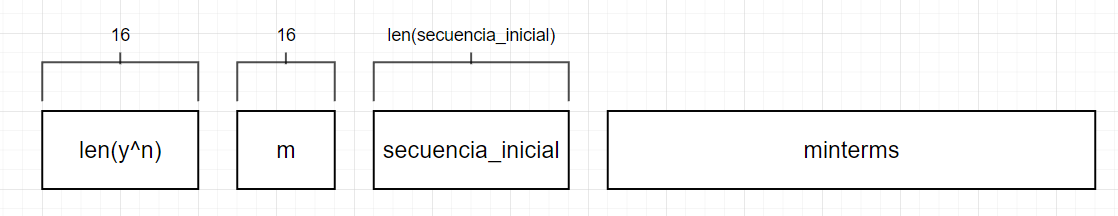
\includegraphics[width=\textwidth,keepaspectratio]{img/nlfsrformat_01.png} .
    \parbox{\linewidth}{\centering Formato .nlfsr}
    \label{fig:mi_imagen}
\end{figure}

\noindent El primer segmento del archivo es la longitud de la cadena original ($y^n$), contenido en 16 bits. Estos 16 bits limitan el tamaño de la secuencia a comprimir en este formato, a una secuencia de longitud máxima 65536. Este límite es arbitrario, pero una vez se haya leído toda la explicación del formato entenderéis que no es difícil adaptarlo para cadenas más largas.  El segundo segmento es la complejidad no lineal $m$ de $y^n$ contenida también en 16 bits (o 2 Bytes). El tercer segmento es la secuencia inicial que mide $m$ bits. Y el cuarto segmento es una lista de \textit{minterms}, aquí tenéis una representación de como se representa un \textit{minterm}.
\\
\begin{figure}[h] % El [H] asegura que la imagen esté exactamente en ese lugar en el documento.
    \centering
    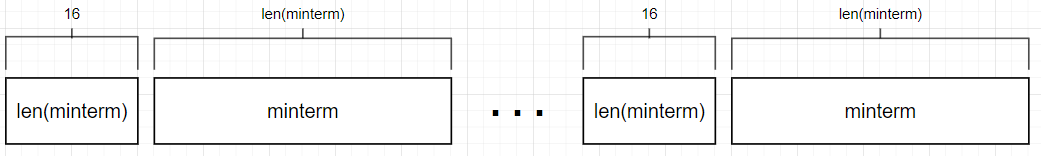
\includegraphics[width=\textwidth,keepaspectratio]{img/nlfsrformat_02.png} % La imagen se ajustará al ancho del texto, manteniendo la proporción.
    \parbox{\linewidth}{\centering Lista de minterms en formato .nlfsr}
    \label{fig:mi_imagen} % Etiqueta para referenciar la imagen en el documento.
\end{figure}
\noindent Cada \textit{minterm} consta de un primer segmento en el que se indica el numero de variables de ese producto de literales lógicos, o dicho de otra manera la longitud. Cada bit del \textit{minterm} representara el estado de ese literal en el producto, si su valor es 1 eso significa que el literal se encuentra negado, por otro lado, si es 0, significará que es positivo. De esta manera, conseguimos almacenar toda la información consumiendo el mínimo numero de bytes posibles. \\\\
La longitud del propio \textit{minterm} actuando como delimitador entre \textit{minterms}, nos permite saber hasta donde tenemos que leer cuando haya que decodificar el archivo .nlfsr. Es importante aclarar, que no se pueden utilizar delimitadores fijos en este caso, como sí se en algunos protocolos de red, ya que toda secuencia podría estar dentro del minterm, y eso haría que se mezclasen los datos con las delimitaciones, lo cual provocaría errores en el momento de la lectura.
\\\\
He hecho unas gráficas para que se pueda ver la diferencia entre guardar un nlfsr de una secuencia con la misma estructura del formato .nlfsr pero usando caracteres ASCII, y utilizar el formato .nlfsr. Aquí tenéis las gráficas sin que se haya utilizado ningún algoritmo de compresión después. 
\begin{figure}[h] % El [H] asegura que la imagen esté exactamente en ese lugar en el documento.
    \centering
    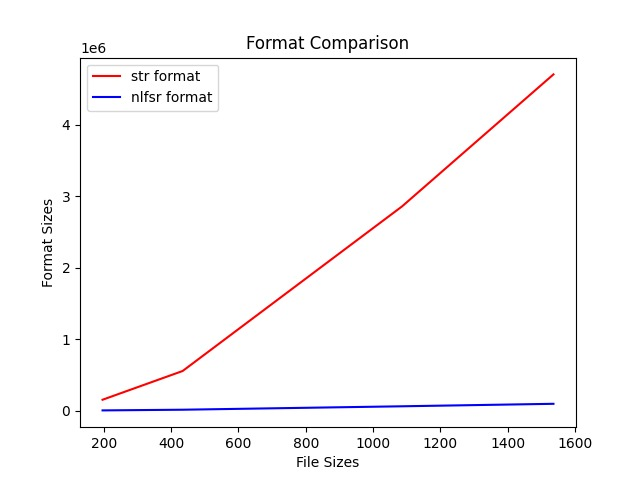
\includegraphics[width=0.8\textwidth,keepaspectratio]{img/format_comparison_graph.jpeg}
    \parbox{\linewidth}{\centering Comparación tamaños formatos}
    \label{fig:mi_imagen} 
\end{figure}
%Encriptación distribuida,
% \subsection{Potenciales aplicaciones del formato nlfsr} (posible seccion)
% Encriptación minimizada distribuida,
\newpage
\section{Minimización de ESOP}
La minimización de expresiones de operaciones AND-OR cuenta con muchos algoritmos que hacen un buen trabajo, sin embargo la minimización de ESOP resulta ser mucho más compleja o al menos, no se han desarrollado algoritmos del mismo calibre. Pero primero, definamos que es todo esto.\\\\
A la forma de la función FSR, se la conoce como ESOP (\textit{Exclusive Sum Of Products}). Una formula lógica con esta forma, tan solo puede tener dos operaciones: XOR (suma) y AND (multiplicación). Minimizar una fórmula ESOP, significa encontrar una formula de menor tamaño que tenga la misma tabla de verdad, o el mismo mapa de Karnaugh; en definitiva, que sean equivalentes.Aquí tenéis un ejemplo de un ESOP y su minimización, aunque más tarde veremos la teoría que hay detrás.
\\\\
\noindent
\begin{minipage}{0.5\textwidth}
    \centering
    \begin{karnaugh-map}[4][2][1][$X_1X_0$][$X_2$]
        \minterms{1, 5, 6, 7}
        \maxterms{0, 2, 3, 4}
    \end{karnaugh-map}
\end{minipage}
\begin{minipage}{0.5\textwidth}
    \[
    f(X_0, X_1, X_2) = X_0X_1 \oplus X_1X_2 \oplus X_2
    \]
\end{minipage}%
\\
Ahora trataremos de encontrar una equivalencia entre $X_1X_2 \oplus X_2$ y un cubo formado por estos literales. Encontramos que
\\\\
\noindent
\begin{minipage}{0.5\textwidth}
    \centering
    \begin{karnaugh-map}[2][2][1][$X_1$][$X_2$]
        \minterms{1}
        \maxterms{0,2, 3}
    \end{karnaugh-map}
\end{minipage}
\begin{minipage}{0.5\textwidth}

     \begin{align*}
          f'(X_1, X_2) =  X_1X_2 \oplus X_2 \\
     z(X_1, X_2) =  X'_1X_2 \\
     f' = z
     \end{align*}
\end{minipage}%
%\newpage
Y sabiendo esto, sustituimos en la formula original y nos queda un ESOP minimizado

\[f_{min} = X_0X_1 \oplus X'_1X_2\]
\\
La \textit{Suma Exclusiva de Productos} se ha estudiado desde 1925 [Paper original], el artículo más reciente que he encontrado respecto a este tema es []. En este describen un algoritmo en el que mediante transformaciones de cubos, expresiones pseudokronecker, reescritura de términos \cite{brand1993minimization}, y estructuras de datos como BDD (Binary Decision Diagram). Nuestra aproximación al problema en este proyecto será mucho más sencilla pero haber leído todos estos artículos sobre el tema, me ha hecho entender más en profundidad lo complejo que es.
\\\\
A pesar de no hacer una implementación como la de [Heuristic Minimiza], en esta sección tomaremos prestada la teoría que elabora el artículo sobre los cubos que forman los ESOP. Definiremos como "cubo" a cada producto del ESOP. Definiremos como distancia entre cubos, el numero de variables que aparecen de distinta "forma" respecto al otro cubo. Una variable puede aparecer en un cubo de tres maneras: en positivo, negada, o no aparecer. Por ejemplo, un cubo $ab$ tiene distancia 1 respecto a un cubo $ab'$. Lo último, que creo que se debe tener en cuenta del articulo para la posible mejora de nuestro algoritmo, son dos proposiciones 
\begin{tcolorbox}
\textbf{Proposición 1:}\\
Si añades el mismo cubo dos veces a cualquier ESOP, la función no cambiará. \\
\textbf{Proposición 2:}\\
La suma de dos cubos con distancia 1 se puede representar en un solo cubo. 
\end{tcolorbox}
%\noindent En el ejemplo anterior aplicamos la segunda proposición para minimizar la función.





\subsection{Enumeración explicita para encontrar el ESOP de N variables de menor longitud}
¿Y si en lugar de encontrar el mínimo para una fórmula en concreto, encontramos el mínimo de símbolos que debe de tener una fórmula para todos los resultados posibles dada una formula (o ESOP) de n variables de entrada? Pues bien, esto es justo lo que hace nuestro pequeño algoritmo. En lo que sigue veremos paso a paso en que consiste. El primer paso que debemos entender es como conseguimos representar todas las formulas posibles de n variables con m simbolos, pudiendo ser cada símbolo, o bien, un XOR, o bien, un AND. La estructura que utilizamos para lograrlo es muy sencilla, es una lista de enteros. Pero tiene un truco, y es que el 0 representa el XOR o la suma, el 1 representa la operación AND o la multiplicación, y el 2 representa la negación. Cualquier entero $i > 2$ representa una variable de entrada $X_{i - 3}$. Con este sistema de representación en el que cualquier fórmula puede ser representada por una lista o cadena de enteros en la que cada posición tiene un entero $i$, $0 <= i < n+3$ de longitud, $m+(m+1)$, siendo $n$ el numero de variables de la fórmula y $m$, el numero de símbolos(XOR, AND) que puede tener la fórmula. \\\\
Para entender mejor el sistema, pondré los siguientes ejemplos. Teniendo una formula $X_0 * X_2 * X_3 + X_0$ y otra formula $X'_0 + X_1 * X_3 + X_4$, estas son sus representaciones con este sistema.
\begin{align*}
X_0 * X_2 * X_3 + X_0 = [0, 1, 3, 1, 5, 6, 3] \\
X'_0 + X_1 * X_3 + X_4 = [1, 0, 2, 3, 4, 0, 6, 7]
\end{align*}
El cálculo del numero de posibles resultados para una formula de n variables de entrada es
\[k = 2^{2^{n}}\]
Ahora debemos encontrar para cada posible resultado del conjunto de posibles resultados de tamaño k, una formula que satisfaga ese resultado. Para ello lo que haremos, será generar todas las combinaciones con repetición del conjunto $\{0,1, ..., n + 3 - 1\}$ de longitud $p$, definimos al conjunto de todas las combinaciones como $g^{(n+3-1)^p}$, cada elemento de $g$ será una posible combinación de tamaño $p$. Es importante decir que, $p$ determinará el numero de posibles símbolos que pueden haber en la fórmula. \\\\
\newpage
Es cierto que habrá algunas combinaciones que no tendrán sentido sintáctico en esta gramática que hemos creado. Por ejemplo $[2, 2, 2, 2, 2, 2, 2]$, no representa ninguna fórmula. Para distinguir entre las listas que tienen sentido de las que no, hemos escrito una función recursiva que crea una cadena de texto o \textit{string} en base a la lista. Aquí tenéis el pseudocódigo, también podéis leer el código real escrito en Python en \href{https://github.com/domingoUnican/TFGPedroCastro/blob/main/code/logicformula_solver/logicform_solver.py}{logicformulasolver.py}.
\begin{algorithm}
\caption{Algoritmo intListToStringFormula(f)}\label{alg:five}
\KwData{$f$ = lista de enteros}
\KwResult{Función lógica en formato string}
\If{\texttt{isNotEmpty(f)}} {
    $val \gets \texttt{f.pop()}$\tcp*{pops last int from f}
    
    \If{\(val == 0\)} {
        \texttt{return stringFormula(f) + '+' + stringFormula(f)}\;
    }
    \If{\(val == 1\)} {
        \texttt{return stringFormula(f) + '*' + stringFormula(f)}\;
    }
    \If{\(val == 2\)} {
        \texttt{return 'not' + stringFormula(f)}\;
    }
    \texttt{return 'x' + (val - 3)}\;
}
\texttt{return 'S'}\;
\end{algorithm}

\noindent El siguiente paso, es escribir la función para calcular cuantos posibles resultados se generan para un numero de variables dado y una longitud de la cadena de lista de enteros dada. Que lo único que hace es para cada cadena de enteros válida (validada con la función del pseudocódigo escrita encima de este párrafo). Prueba todas las posibles combinaciones de las variables de entrada de la función, es decir si por ejemplo, es una función de 3 variables de entrada probara las $2^3$ combinaciones. Recopilará todos los resultados y hará una lista con ellos. La intentará sumar a un set, la cual se sumará en función del hash calculado a esa lista internamente por Python.\\\\ Una vez se han agotado todas las combinaciones de listas de enteros ("formulas lógicas"), se comparará la longitud del set con el número de posibles resultados $k$; si estos coinciden es que hemos encontrado el tamaño mínimo de la lista de enteros para generar todas las formulas necesarias que coinciden con todos los resultados posibles. \\ 
\newpage
\noindent Aquí tenéis dos gráficas creadas con la librería \textit{matplotlib}, en el eje $X$ la primera fila es el tiempo que ha tardado en ejecutar el algoritmo, y la segunda fila es el tamaño de la lista de enteros. El eje $Y$ representa el numero de posibles resultados retornados por el algoritmo.

\begin{figure}[h!]
    \centering
    \begin{minipage}{0.5\textwidth}
        \centering
        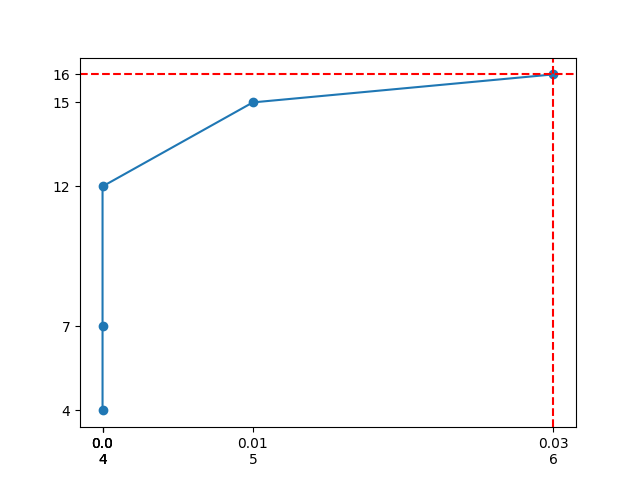
\includegraphics[width=\linewidth]{img/2_variables.png}
        \parbox{\linewidth}{\centering ESOP de 2 variables de entrada}
    \end{minipage}%
    \begin{minipage}{0.5\textwidth}
        \centering
        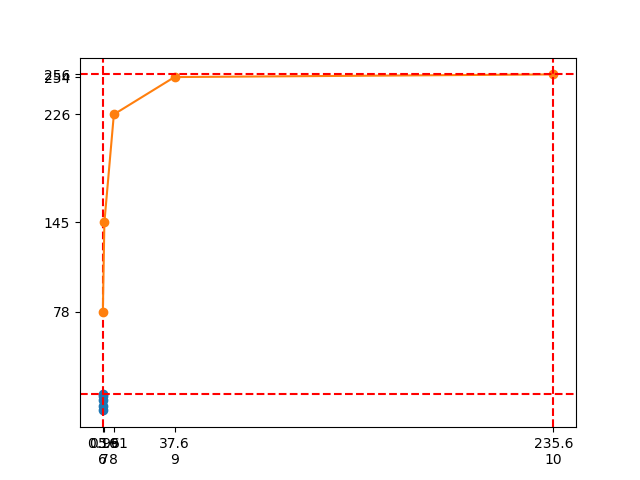
\includegraphics[width=\linewidth]{img/3_variables.png}
        \parbox{\linewidth}{\centering ESOP de 3 variables de entrada}
    \end{minipage}
    \vspace{1em} % Espacio entre las filas de imágenes

    \begin{minipage}{0.5\textwidth}
        \centering
        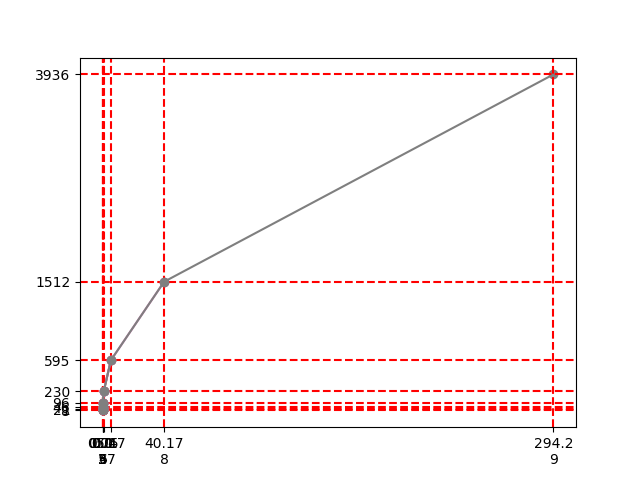
\includegraphics[width=\linewidth]{img/4_variables.png}
        \parbox{\linewidth}{\centering ESOP de 4 variables de entrada}
    \end{minipage}
\end{figure}

\noindent Como vemos en las gráficas, el algoritmo converge en ambos casos es decir, encuentra todas las listas de enteros que satisfacen los $k$ posibles resultados para ESOP de $n$ variables. Sin embargo, a partir de ESOPs de 4 variables debido a la complejidad temporal del algoritmo, se tarda mucho en que el algoritmo converja y empeora conforme el número de variables aumenta, ya que la complejidad temporal de nuestro algoritmo es de $O((n+3)^p * 2^n)$. Con mi procesador, en 10 minutos consigue calcular la función hasta $p = 9$.
\\\\
Para calcular las combinaciones en el código original, hemos usado la librería \textit{itertools}, y en concreto la función \textit{product}, ya que fue una recomendación de mi tutor, Domingo. Este modulo de Python genera sus funciones, utilizando Cython para después crear módulos utilizables desde Python, pero escritos en C. Sentí cierta curiosidad, por como sería hacer un programa en C que calcule todas las combinaciones tal y como lo hace \textit{itertools}.\\\\
Así que me puse manos a la obra, y escribí dos versiones una secuencial \href{https://github.com/domingoUnican/TFGPedroCastro/blob/main/code/list_product/list_product.c}{secuencial.c}. y otra paralelizada con \textit{OpenMP} \href{https://github.com/domingoUnican/TFGPedroCastro/blob/main/code/list_product/list_product_parallel.c}{paralelo.c}. Si habéis leído el código sabréis que lo hago todo sobre un solo array, lo escribí así por temas de la localidad de los valores guardados. En mi \textit{hardware}, el código secuencial resultó ser un poco más lento que el de \textit{itertools}, sin embargo, para mi sorpresa el código paralelizado sí me dio mejores resultados, incluso superando a la función del módulo de Python. Si bien, es cierto que Python está "capado" por el GIL (Global Interpreter Locker), ya que a pesar de contar con módulos que ofrecen funciones de "multithreading" no se consigue en ningún momento una paralelización real, considero que los datos siguen siendo interesantes, aquí tenéis una gráfica.

\begin{figure}[h] % El [H] asegura que la imagen esté exactamente en ese lugar en el documento.
    \centering
    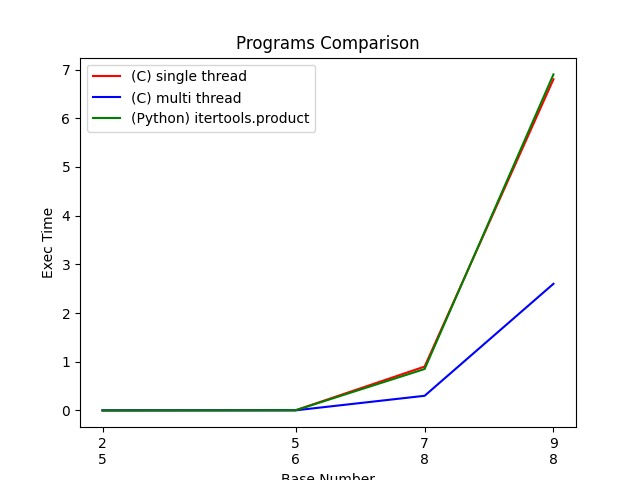
\includegraphics[width=0.9\textwidth,keepaspectratio]{img/programs_comparison_graph.jpeg}
    \parbox{\linewidth}{\centering Comparación tamaños formatos}
    \label{fig:mi_imagen} 
\end{figure}
\noindent El eje Y es el tiempo de ejecución en segundos, y el eje X tiene 2 listas de valores, la lista más cercana al eje es el cardinal del conjunto sobre el que se calculan todas las posibles combinaciones. y el tamaño de la lista es el número de debajo. Cabe destacar que para un conjunto de 10 elementos y un tamaño de lista 8, mi sistema operativo (Debian \textit{bookworm}) mataba el proceso de Python. Sin embargo, para los mismos parámetros mis programas escritos en C, tanto el secuencial como el paralelo, registraron 16.8 y 5.8 segundos respectivamente. Evidentemente con parámetros más altos tenía problemas de memoria debido a mi \textit{hardware} limitado.